%%%%%%%%%%%%%%%%%%%%%%%%%%%%%%%%%%%%%%%%%%%%%%%%%%%%%%%%%%%%%%%%%%%%%%%%%%%%%%%%%%%%%%%%%%%%%%%%%%%%%%
% Plantilla básica de Latex en Español.
%
% Autor: Andrés Herrera Poyatos (https://github.com/andreshp)
%
% Es una plantilla básica para redactar documentos. Utiliza el paquete fancyhdr para darle un
% estilo moderno pero serio.
%
% La plantilla se encuentra adaptada al español.
%
%%%%%%%%%%%%%%%%%%%%%%%%%%%%%%%%%%%%%%%%%%%%%%%%%%%%%%%%%%%%%%%%%%%%%%%%%%%%%%%%%%%%%%%%%%%%%%%%%%%%%%

%-----------------------------------------------------------------------------------------------------
%	INCLUSIÓN DE PAQUETES BÁSICOS
%-----------------------------------------------------------------------------------------------------

\documentclass{article}

% Lenguaje
\usepackage[spanish,es-noquoting, es-tabla, es-lcroman]{babel}
\usepackage[utf8]{inputenc}
\selectlanguage{spanish}

% fuente mono
\usepackage{fontspec}
\setmonofont{Inconsolata}

% Matemáticas
\usepackage{amsthm}
\usepackage{amsfonts}
\usepackage{amsmath}
\usepackage{tikz-cd}
\theoremstyle{plain}
\newtheorem{theorem}{Teorema}
\newtheorem{proposition}{Proposición}
\newtheorem{lemma}{Lema}
\newtheorem{corollary}{Corolario}
\theoremstyle{definition}
\newtheorem{definition}{Definición}
\theoremstyle{remark}
\newtheorem*{remark}{Nota}
\renewcommand*{\proofname}{Demostración}

\DeclareMathOperator{\Inv}{Inv}
\DeclareMathOperator{\fr}{Fr}
\DeclareMathOperator{\rad}{Rad}
\DeclareMathOperator{\dist}{dist}

\newcommand{\abs}[1]{\ensuremath\left\vert #1 \right\vert}
\newcommand{\norm}[1]{\ensuremath\left\Vert #1 \right\Vert}
\newcommand{\normt}[1]{\ensuremath\left\vert\kern-0.25ex\left\vert\kern-0.25ex\left\vert #1 \right\vert\kern-0.25ex\right\vert\kern-0.25ex\right\vert}

% Corrige el espacio previo a las definiciones
\makeatletter
\def\thm@space@setup{%
  \thm@preskip=\parskip \thm@postskip=0pt
}
\makeatother

% Fuente
\usepackage{courier}
\usepackage{microtype}


% ----
% Estilo de página
%----
% Paquetes para el diseño de página:
\usepackage{fancyhdr}               % Utilizado para hacer títulos propios.
\usepackage{lastpage}               % Referencia a la última página. Utilizado para el pie de página.
\usepackage{extramarks}             % Marcas extras. Utilizado en pie de página y cabecera.
\usepackage[parfill]{parskip}       % Crea una nueva línea entre párrafos.
\usepackage{geometry}               % Asigna la "geometría" de las páginas.

% Se elige el estilo fancy y márgenes de 3 centímetros.
\pagestyle{fancy}
\geometry{left=3cm,right=3cm,top=3cm,bottom=3cm,headheight=1cm,headsep=0.5cm} % Márgenes y cabecera.
\fancyhf{}

% Espacios en el documento:
\linespread{1.1}                        % Espacio entre líneas.
\setlength\parindent{0pt}               % Selecciona la indentación para cada inicio de párrafo.

% Cabecera del documento. Se ajusta la línea de la cabecera.
\renewcommand\headrule{
	\begin{minipage}{1\textwidth}
	    \hrule width \hsize
	\end{minipage}
}

% Texto de la cabecera:
\lhead{\docauthor}                          % Parte izquierda.
\chead{}                                    % Centro.
\rhead{\subject \ - \doctitle}              % Parte derecha.

% Pie de página del documento. Se ajusta la línea del pie de página.
\renewcommand\footrule{
\begin{minipage}{1\textwidth}
    \hrule width \hsize
\end{minipage}\par
}

\lfoot{}                                                 % Parte izquierda.
\cfoot{}                                                 % Centro.
\rfoot{Página\ \thepage\ de\ \protect\pageref{LastPage}} % Parte derecha.


% ----
% PORTADA
% ----

% Estilo
\usepackage{title1}

% Título y autores
\newcommand{\doctitle}{Disco de Poincaré}
\newcommand{\docsubtitle}{}
\newcommand{\docdate}{1 \ de \ Enero \ de \ 2015}
\newcommand{\subject}{Geometría hiperbólica}
\newcommand{\docauthor}{M. Gómez, E.M. González, D. Melero, M. Román}
\newcommand{\docaddress}{Universidad de Granada}
\newcommand{\docemail}{}

% Resumen
\newcommand{\docabstract}{En la geometría hiperbólica, el quinto postulado de Euclides es sustituido por el axioma de Lobachevsky.}

\begin{document}

\maketitle

% Profundidad del Índice
%\setcounter{tocdepth}{1}
\newpage
\tableofcontents
\newpage

\section{Introducción}

La geometría hiperbólica es un modelo de geometría que satisface sólo
los cuatro primeros postulados de la geometría euclidiana. Aunque es
similar en muchos aspectos y muchos de los teoremas de la geometría
euclidiana siguen siendo válidos en geometría hiperbólica, no se
satisface el quinto postulado de Euclides sobre las paralelas.

Desde la antigua Grecia se realizaron esfuerzos por deducir el quinto
postulado de Euclides referente a las paralelas de los otros
cuatro. Uno de los intentos más amplios y ambiciosos fue el de
Giovanni Gerolamo Saccheri en el siglo XVIII quien,
contradictoriamente creó lo que podríamos considerar modelo incipiente
de geometría hiperbólica. Sin embargo, Saccheri creyó que no era
consistente y no llegó a formalizar todos los aspectos de su
trabajo. También Johann Heinrich Lambert encontró algunas fórmulas
interesantes referentes a lo que hoy llamaríamos triángulos de la
geometría hiperbólica, probando que la suma de los ángulos es siempre
menor que 180º, la fórmula de Lambert establecía que para uno de estos
triángulos se
cumplía: $$\pi-\alpha-\beta-\gamma=DA_{\alpha,\beta,\gamma},$$ donde
$\alpha,\beta,\gamma$ son los ángulos del triángulo,
$A_{\alpha,\beta,\gamma}$ es el área del triángulo y C es una
constante de proporcionalidad positiva relacionada con la curvatura
del espacio hiperbólico donde se haye inmerso el triángulo.

Más adelante Carl Friedrich Gauss trabajó en un modelo similar pero no
publicó sus resultados. En los años 1820 dos jóvenes matemáticos que
trabajaban de modo independiente, János Bolyai y Nikolai Ivanovich
Lobachevsky, publicaron sus modelos por los cuales establecían la
posibilidad de un tipo de geometría alternativa, totalmente
consistente, que es el que conocemos como geometría hiperbólica.

Existen varios modelos de geometría hiperbólica: la representación de
Klein, el modelo del disco de Poincaré y el modelo de Lorentz o del
hiperboloide.

Curiosamente los dos primeros modelos fueron propuestos y publicados
originalmente por Eugenio Beltrami en 1968, sin embargo, alcanzaron
notoriedad por el uso que tanto Felix Klein como Henri Poincaré
hicieron de ellos, estos dos modelos son modelos de la geometría
hiperbólica de dos dimensiones, y son generalizables a más
dimensiones.

La representación de Klein, también conocido como el modelo proyectivo
del disco ó modelo de Beltrami-Klein, usa el interior de un círculo
como plano hiperbólico, y las cuerdas como líneas del círculo.

El modelo de Poincaré usa también el interior de un círculo plano, y
en él las líneas rectas de la geometría hiperbólica vienen
representadas por arcos de circuferencia que cortan el borde del
crículo plano en ángulo recto.

\section{Modelo del hiperboloide}

Este modelo de geometría hiperbólica se basa en la forma cuadrática de
Lorentz: $$L(x,y,z)=x^2+y^2-x^2.$$ Si pensamos en esta forma
cuadrática como una norma, tenemos vectores distintos de cero con
norma cero e incluso norma negativa. Esto nos da una clasificación de
los vectores: \begin{enumerate}
\item{Vectores espaciales:$x\in\mathbb{R}^3$ tal que $L(x)>0$}
\item{Vectores temporales:$x\in\mathbb{R}^3$ tal que $L(x)<0$}
\item{Vectores luminosos:$x\in\mathbb{R}^3$ tal que $L(x)=0$}
 \end{enumerate}

 Definimos $$\mathbb{H}^2=\{x\in\mathbb{R}^3 | L(x)=-1,x(0,0,1)>0\},$$
 como vemos esta es la hoja superior de un hiperboloide de dos
 hojas. Como sabemos es una superficie y por tanto localmente
 homeomorfo a un plano. Lo llamamos plano hiperbólico.

\subsection{Rectas}

Las rectas en el plano hiperbólico se definen como las intersecciones
de $\mathbb{H}$ con planos que pasan por el origen. Las llamamos
rectas hiperbólicas.

\section{Disco de Poincaré}

\subsection{Métrica en el disco de Poincaré}

\subsubsection{Distancia}
Si $u,v$ son dos vectores del espacio euclídeo $\mathbb{R}^n$,ambos
con norma inferior a $1$, podemos definir un invariante isométrico de
la siguiente manera:
$$\delta (u,v)=2\frac{\norm{u-v}^2}{(1-\norm{u}^2)(1-\norm{v}^2)} ,$$
donde $\norm{.}$ representa la norma euclídea usual. Definimos la
función distancia como: $$d(u,v)=arccosh(1+\delta(u,v)).$$ Esta
función de distancia está definida para cualesquiera dos vectores de
norma inferior a uno, y el conjunto de tales vectores forman un
espacio métrico que es un modelo de espacio hipérbólico de curvatura
constante -1, como sabemos el disco de Poincaré.

Como bien sabemos la funcion arccosh es creciente, luego cuanto mayor
sea $\delta (u,v)$ mayor será la distancia que separa $u$ y $v$. Ahora
bien, si acercamos uno de los dos vectores $u$ o $v$ hacia la frontera
del disco, su norma se acercará a uno y por tanto la función $\delta$
crecerá y como consecuencia la función distancia también. Es decir, si
tenemos dos vectores,uno suficientemente lejos de la frontera y vamos
acercando el otro a la frontera, la distancia entre los dos crecerá.

\newpage

Por ejemplo, en la siguiente imagen todos los puntos están a la misma
distancia del punto A:

\begin{figure}[h]
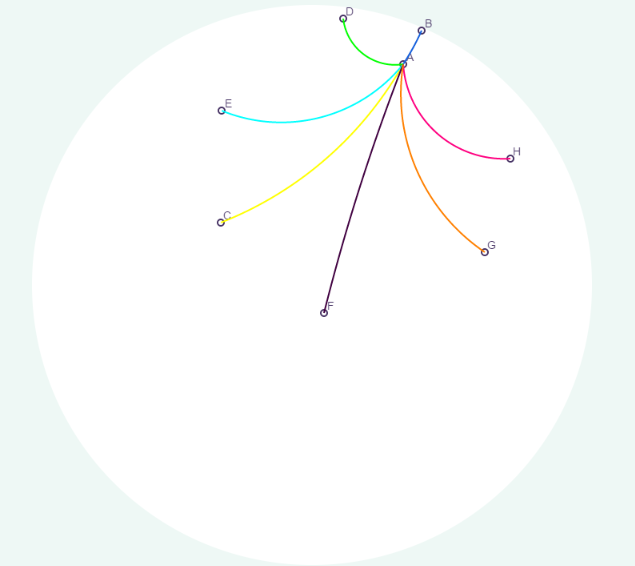
\includegraphics{Distancias.png}
\end{figure}

Veamos también como sería una circunferencia con centro A un punto
cercano a la frontera y de radio, por ejemplo, 4:

\begin{figure}[h]
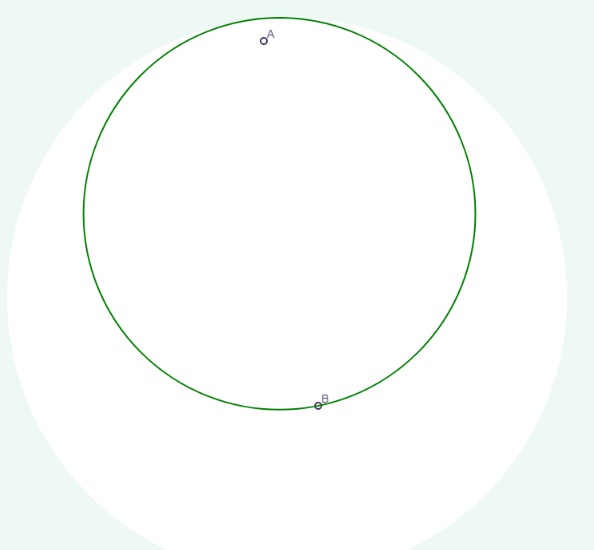
\includegraphics{Circunferencia.png}
\end{figure}

\newpage

\subsubsection{Rectas}

Dados ahora dos puntos vamos a ver como es la recta que pase por los
dos puntos dados. En el modelo del disco de Poincaré, las rectas del
plano se definen por arcos de circunferencias con ecuaciones de la
forma: $$x^2+y^2+ax+by+1=0,$$
que es la forma general de una circunferencia que corta ortogonalmente al disco unidad.\\
Dados dos puntos u y v en el disco que no estén en un diámetro, se
puede resolver para el círculo de esta forma pasando por ambos puntos,
y obtener
$$x^{2}+y^{2}+{\frac {u_{2}(v_{1}^{2}+v_{2}^{2})-v_{2}(u_{1}^{2}+u_{2}^{2})+u_{2}-v_{2}}{u_{1}v_{2}-u_{2}v_{1}}}x+{\frac {v_{1}(u_{1}^{2}+u_{2}^{2})-u_{1}(v_{1}^{2}+v_{2}^{2})+v_{1}-u_{1}}{u_{1}v_{2}-u_{2}v_{1}}}y+1=0.$$

\subsubsection{Ángulos}
Los ángulos son euclidianos. Si tenemos dos líneas hiperbólicas, cada
una de ellas es un arco de circunferencia, luego la medida del ángulo
que se forma entre las dos líneas hiperbólicas es el ángulo que forman
las tangentes de las circunferencias en el punto en que éstas se
intersecan.

\subsubsection{Relación con el modelo del hiperboloide}
Este modelo se relaciona con el modelo del hiperboloide
proyectivamente. Dado un punto $(t, x_1,x_2)$ sobre la hoja superior
de un hiperboloide del modelo del hiperboloide, se define un punto del
modelo del disco de Poincaré, que se puede proyectar sobre el plano
t=0,el resultado es el correspondiente punto del disco de Poincaré.
Para las coordenadas cartesianas $(t,x_1,x_2)$ del hiperboloide e
$(y_1,y_2)$ del plano, las fórmulas de conversión son :

$$y_{i}=\frac {x_{i}}{1+t}$$
$$(t,x_{i})=\frac {(1+\sum {y_{i}^{2}},2y_{i})}{1-\sum {y_{i}^{2}}}$$


\section{Referencias}
\begin{thebibliography}{9}

\bibitem{gelfand63}
  Gelfand, I.M.; Minlos, R.A.; Shapiro, Z.Ya. (1963),
  Representations of the Rotation and Lorentz Groups and their Applications,
  New York: Pergamon Press.


\end{thebibliography}

\end{document}
